\section{Background and Related Works}
\label{sec:bg}

\subsection{Topology-based analysis}
% \subsection{Topological Analysis}
% Morse theory describes the topology of differentiable functions on a manifold, $f:M\rightarrow{\rm I\!R}$. 
 Morse theory describes the topology of differentiable functions on a manifold~\cite{Milnor63}. The critical points of a function $f$ occur where the gradient vanishes with index equal to the number of negative eigenvalues of the Hessian. Integral lines are paths that are tangent to $\nabla f$, do not intersect, and have lower and upper limits at critical points, called the origin and destination, respectively. The \textit{ascending} and \textit{descending manifold} of a critical point is the union of integral lines originating, and terminating at that point, respectively. For $f$ defined on a $d$-dimensional manifold, an index-$i$ critical point has a $d-i$ dimensional ascending manifold and $d$-dimensional descending manifold. A function is Morse-Smale~\cite{Sma61a, Sma61b}  if all ascending and descending manifolds intersect transversally, or not at all. The intersections of all ascending and descending manifolds forms a cell complex called the Morse-Smale complex. Each $d$-dimensional cell of the complex, called a \textit{partition}, is composed of points whose integral lines originate and terminate at the same minimum-maximum pair. Figure~\ref{fig:msc-overview} Shows the critical points, integral lines, and cells of the Morse-Smale complex of a 2-dimensional scalar function. 

A Morse-Smale complex is simplified by repeated cancellation of critical point pairs that differ in index by one~\cite{edelsbrunner03}. Persistent homology orders cancellations by increasing difference in function value~\cite{edelsbrunner02}. In the Morse-Smale complex, a cancellation is realized by removing a pair of critical points and merging their ascending and descending manifolds with their neighbors~\cite{Gyulassy06tvcg2, Gyulassy2012}. For $d>2$ a 1-saddle that separates distinct minima is called a split saddle, and a $d-1$-saddle that separates distinct maxima is called a merge saddle. When cancelling a merge or split saddle with an extremum, the effect on the Morse-Smale complex is to merge partitions separated by the $d-1$-manifold emanating from the saddle. As a cancellation corresponds to a \textit{local} change in $f$, and corresponding \textit{local} change to the structure of the Morse-Smale complex, independent cancellations can be organized into a \textit{persistence hierarchy}, a directed graph whose arrows local cancellation indicate order dependency~\cite{bremer04}. The subset of cancellations between extrema and split and merge saddles turns the persistence hierarchy into a rooted tree~\cite{Tierny2012}. This tree interpretation motivates tree representation of merging partitions, and enables the overall approach of displaying multi-dimensional persistence hierarchies.  

Morse-Smale complexes, merge trees, contour trees~\cite{carr03}, and Reeb graphs~\cite{pascucci07} all encode aspects of the topology of scalar functions, and have been used successfully to define and compute features in many application domains~\cite{Bremer09tvcg, TopoMS}. While most methods employ persistent homology~\cite{edelsbrunner02} to reason about the features at multiple scales, rarely is the merging of regions directly encoded and visualized. The branch decomposition of contour trees comes close~\cite{Pascucci2009}, encoding persistence and parent-child child relationships in the merging of regions in its structure.   Persistence diagrams~\cite{edelsbrunner02,  edelsbrunner03, Cohen-Steiner07}, and their variants, barcode diagrams~\cite{Ghrist2008}, and persistence landscapes~\cite{bubenik2012statistical} present the persistence pairs and their place in the range of the function, but fail to convey the nesting of topological features.  
% The study of homology for point cloud data across multiple scales, and topological structures such as contour trees and Morse-Smale complexes. 

% Persistence diagram~\cite{edelsbrunner02,  edelsbrunner03, Cohen-Steiner07}, is a point set in the extended plane that encodes the difference in the homology of the sub-level sets of the function. Each point corresponds to a feature and quantifies its importance by the absolute difference between the point’s two coordinates.

% Barcode diagram

% Maybe Persistence landscape and silhouette~\cite{chazal14} used in statistical analysis

A standard approach for selecting an appropriate persistence value, in the context of Morse-Smale complexes, is based on the notion of a persistence graph, which depicts the number of extrema points with respect to the normalized persistence value~\cite{pascucci07, Gerber10}.
%as shown in \autoref{fig:persistence-ui}. 
The expectations are that extrema points with low persistence are most likely due to noise or under sampling. In addition, stable features require a large change in the persistence value before they are removed, leading to visible plateaus in the graph. The persistence graph, however, even when providing clear stable thresholds, does not provide any insights about the underlying function. 

% While in general, a cancellation can create new cells of the complex, in the specific cases of cancelling a minimum with a 1-saddle, and cancelling a maximum with a $d-1$-saddle, the overall effect is to merge the partitions  \textit{persistence hierarchy}.  
% Chazal~\cite{Chazal11}

% \noindent\textbf{outline:}

% Morse theory studies continuous functions on continuous domains. With basic nondegeneracy conditions we get isolated critical points, denseness, nice properties. number of approaches for analysis of Morse functions, including CT, RG, Morse complex, we use latter. a Morse function can be decomposed based on integral lines - forms the cell complex. intersect with other complex = ms complex (with transversal intersections). describe cells of the ms complex - cells are formed by the cross product of ascending 1...d manifolds nad descending 1....d manifolds. the d-dimensional intersections are formed by ascending d-manifolds intersecting with descending d-manifolds. 

% practical computation must operate on a discretized domain. MORE ON MAKING A MESH. there are approaches based on discrete morse theory, PL, etc(do we want to go this route) or just say in high dimensions it is only possible to detect d-manifolds as the origin/destination of steepest paths walking on mesh edges. merge saddles (1 and d-1) occur at the lowest/highest vertices with different labels - are they separated - in theory above 2d they are, but we *could* get a vertex that has both. so define a partition as the set of high-dim points whose paths go from same min to same max. 

% morse function can be repeatedly simplified locally by repeated cancellation of critical points. 
% consider the sub-manifold $\mathbf{M}^+_c = \{ f(p) \geq c \}$ as $c$ is swept from $\infty$ to $-\infty$ - for non-critical values of $f$ it is a $d$-manifold.
% At the maximal value of $f$ on $\mathcal{R}^d$, a component appears. the critical point of each critical value that is passed by $c$ changes the homology of the d-manifold the critical points of the morse function. the critical points that creates a homology class, i.e. component, d-1-cycle, ... , 1-cycle, void. persistent homology describes the life-cycle of homology classes, pairing the critical ppoints that create a class with the one that destroys it. for instance a maximum creates a connected component of $\mathbf{M}^+_c$, where the component merges with a neighboring component happens at a merge saddle. The maximum of the component that appeared later in the sweep is paired with the merge saddle = persistence. 

% Persistence simplification on MS complexes - generally described. for high dim functions, we can only reliably detect extrema and merge saddles. paper describes as merging of manifolds for maxs n mins. as a result, the partitions tha tform the intersections will also just be merged. sequence of cancellations creates nested partitions that can be represented genrally intree (or this in simplification section?) SEE FIG~\ref{fig:msc-overview}


\begin{figure}[tb]
    \begin{center}
    %  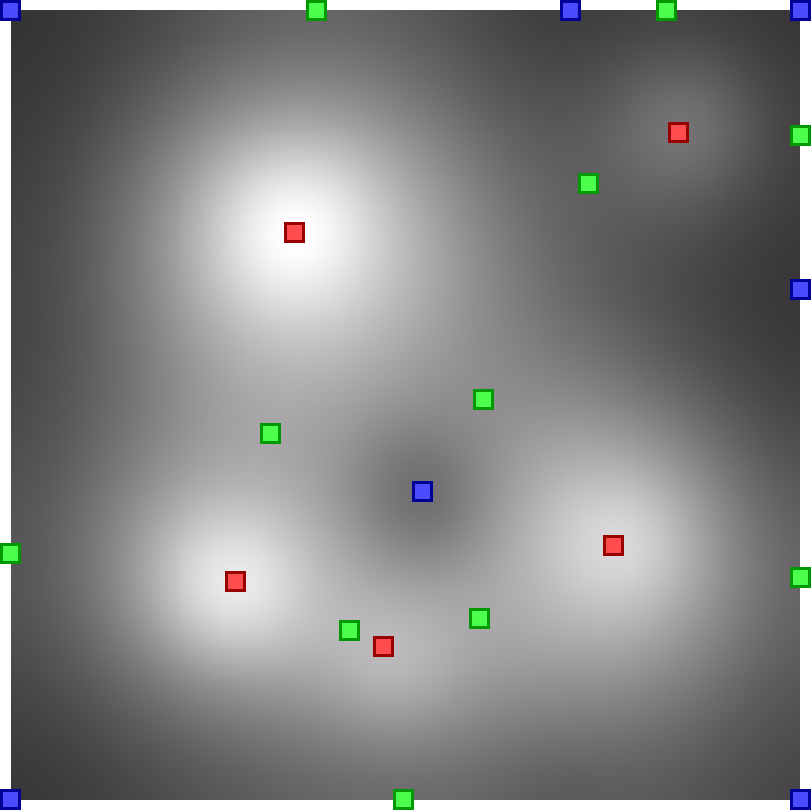
\includegraphics[width=0.241\linewidth]{2020-regulus/figs/msc/im0_0.png}
    %  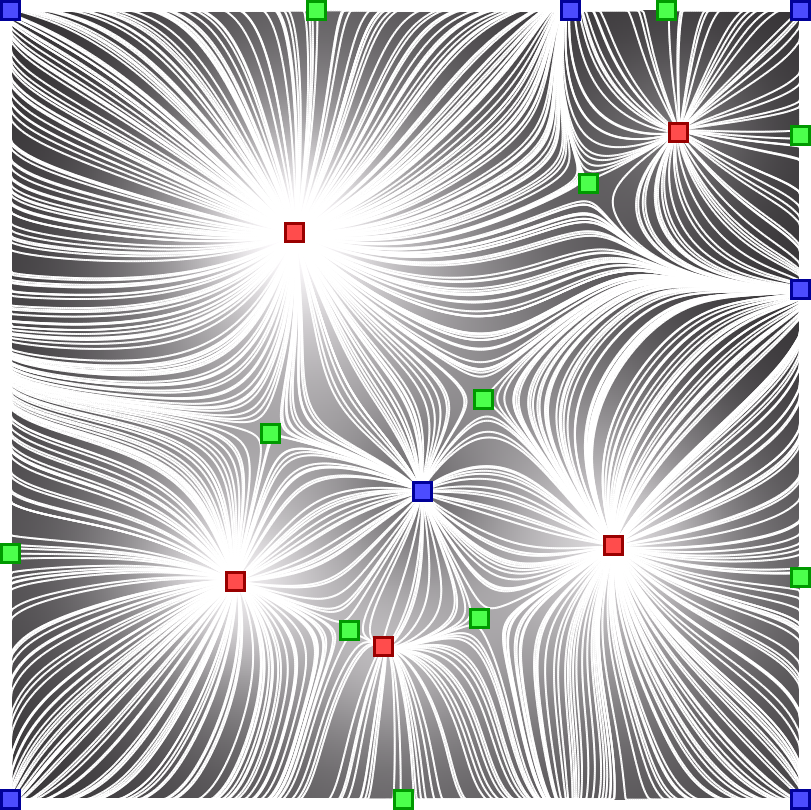
\includegraphics[width=0.241\linewidth]{2020-regulus/figs/msc/im1_0.png}
    %  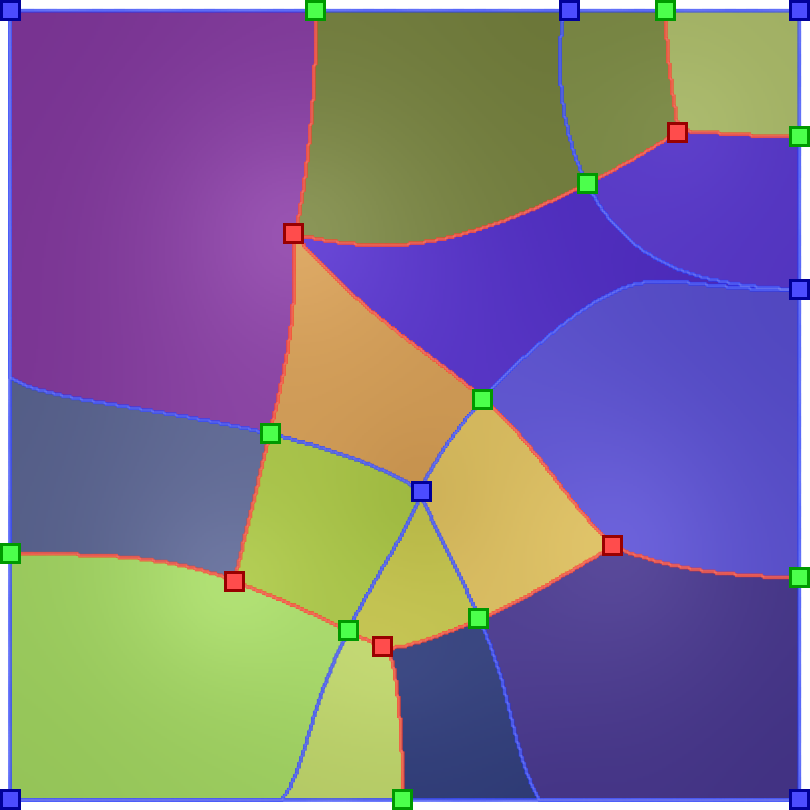
\includegraphics[width=0.241\linewidth]{2020-regulus/figs/msc/im3_0.png}
    %  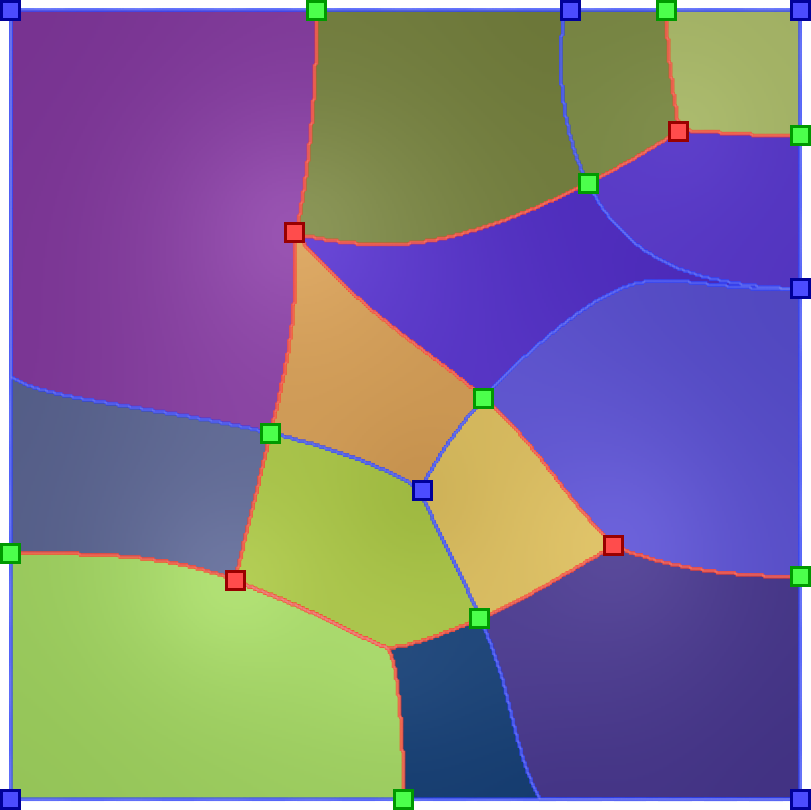
\includegraphics[width=0.241\linewidth]{2020-regulus/figs/msc/im4_0.png}
    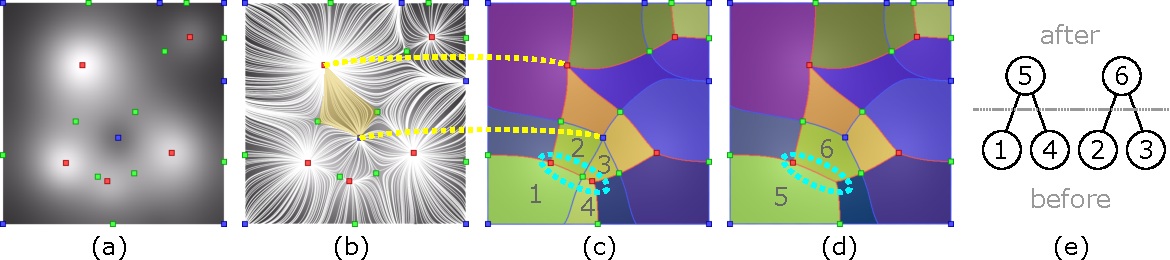
\includegraphics[width=0.99\linewidth]{2020-regulus/figs/msc/mscoveriew2.pdf}
    \vspace{-0.15in}
    \caption{The maxima (red) minima (blue) and saddles (green) of a two-dimensional scalar function (a), are the origin and destination of integral lines (b). A cell of the Morse-Smale complex (c) is formed by integral lines sharing an origin and destination. The 2D patches, called a partitions is highlighted (b,c). Cancellation of a saddle-maximum pair (circled) merges adjacent partitions (c,d); 2,3 merge to 6, and 1,4 merge to 5. The max-saddle cancellation is represented as these merging partition in a \RT (e). }
    \label{fig:msc-overview}
    \end{center}
    \vspace{-.1in}
\end{figure}



% - describe gerber in detail in particular meshing and MS computation and how to get persistence pairs.


% \section{Related Work}

\subsection{Exploring Parameter Spaces}

An important aspect of our work is its applicability to exploration and understanding the functional relationship between multi-dimensional parameter spaces and their derived outputs.
%
HyperMoVal~\cite{Piringer2010} is a system designed for validating support vector regression models against the underlying data.
%
The system employs linked views, local sensitivity information, and model tuning capabilities to allow the user to see not only where the model deviates from the data, but to refine the model interactively until desired criteria are met.

Tuner is a software system designed to help users tune the parameters for image segmentation and combines an automated adaptive sampling phase with a visual exploration stage where stability and sensitivity can be evaluated until the user guides the system to their optimal solution.
%
Berger et al. combine regression models and linked views to provide users with local uncertain-aware sensitivity information that is meant to guide users to interesting regions in their domain.
%
Similar works that focus on such \textit{design steering} methodologies include the works of Matkovic et al.~\cite{Matkovic14, Splechtna15, Matkovic18} where linked views are combined with user-guided adaptive sampling to refine the data and/or models built on the data in areas of interest to the user.

% Similar to these works, we hope to drive user's attention to interesting regions of the topological hierarchy through the use of regression and comparison among models of the data.
% %
% The difference lies in using the Morse-Smale complex and its persistence hierarchy to define \textit{local} models on the data and comparing these local models both within and across levels in the hierarchy.

ParaGlide~\cite{Bergner13} provides an interactive exploration of the parameter space of multidimensional simulation models. The system enable users to define regions in the input space that represent distinct output behavior. The regions are defined manually by the user and are restricted to Cartesian product of ranges in the various input dimensions. 

In contrast to these works, we use Morse-Smale complex to partition the space and  persistence homology to study the space in multiple levels of details. We also fit \textit{local} models on the data and compare and contrast them both within and across levels in the hierarchy.

% He et al.~\cite{He2020} employed a neural network to support parameter space exploration for ensemble simulations that are visualized in situ. They developed a convolutional regression model to learn a mapping from simulation and visualization parameters to visualization results. With the trained model, users can generate new images for different simulation parameters under various visualization settings. The work focuses on synthesizing images rather than of direct analysis of the the data
% Exploring parameter space of simulation models.

\subsection{Visual Exploration}
\label{sec:hd-exploration}

Gerber et al.~\cite{Gerber10} were the first to use Morse-Smale approximation to visualize scalar functions defined on multi-dimensional point cloud data. They created geometric summary of a simplified Morse-Smale complex by using locally weighted regression~\cite{Cleveland88} to fit inverse regression curve in each partition and use dimension reduction to embed them in a 3D display. The curves model the inverse relation from the output value to the input parameters and provide visual cues about each partition such as local and global shape, width, length, and sampling densities. Linked views showed details of the individual partitions and their one/two-dimensional relationships with respect to the output of interest. The 3D visualization is hard to interpret and, as noted by the authors, introduced phantom visual cues such as twists of the curves that did not encode real information. We follow their use of inverse regression curves when depicting details about specific partitions and for generating additional samples but we do not use the 3D view (the sampling is not part of this paper).

Maljovec et al.~\cite{maljovec16} noted that computing all the inverse regression curves in large dataset incurred high overhead and additional manipulation is required to make an aesthetically pleasing visualization where the skeleton connects at the endpoints.
Instead, they employ a more abstract ball and stick style overview that required no additional computation (aside from the Morse-Smale decomposition). Their overview consist of a 2D plot of function value versus persistence value and depicted each partition as a curve between its extrema points. For data fitting, the simpler Morse-Smale regression~\cite{Gerber2011,Gerber2012} strategy were computed on-demand for a specified persistence level. They also used bar charts to compare and contrast the sensitivities and goodness-of-fit of the resultant linear models. Their overview provides a consistent view of where extrema exist in the hierarchy more in line with the work presented herein, but like Gerber's work before them, still only allowed for the visualization of a single persistence level at a time. In contrast to Maljovec et al., we use the inverse regression curves and reduce the computational cost by lazily computing them only for visible partitions and only after reducing the tree.
%
Lastly, neither work shows how a feature merges in the hierarchy and does not provide comparison \textit{across} persistence levels.

% \begin{itemize}
%     \item Gerber 2010 work (this work is based on it). 
%     \begin{itemize}
%         \item Fit an inverse regression curve in each crystal to provide some sort of geometric summary. The curves are 1d curves in $R^d$ and in order to display them, Gerber project the curves down to 3d based on a PCA of all the data points.
        
%         \item Once the user selects a persistence value using (\autoref{fig:persistence-ui}),  Gerber extracts the Morse-Smale representation of the data and then display all the inverse curves (see \autoref{sec:curve-fitting}) for in the partitions (crystals) in the 3D view.
        
%         \item The 3D is problematic because 
%             \begin{itemize}
%                 \item confusing - the axis are not clear and the twists in the curves don't provide any meaningful info
%                 \item to be meaningful the curves suppose to meet at the ends, which require some fiddling with the data. 
%                 \item the curves are not a good representation for coarse partitions that do not have a good linear model. 
%             \end{itemize}
        
%         \item the user can see details only about a single partition at a time
        
%         \item single global refinement (persistence) level based on \autoref{fig:persistence-ui}
    
%     \end{itemize}

%     \item Dan's works. 
%     \begin{itemize}
%         \item Dan uses only linear lines instead of inverse regression curves because they are too expensive to precompute as Gerber did
%         \item Visual comparison of partitions across a single level of a partition using bar charts (compare sensitivities to find similar behaving partitions)
%         \item Fitness view gives a sense of what partitions are sufficiently fitting at a given persistence. Can also be used to identify how many dimensions are necessary for fitting.
%     \end{itemize}
% \end{itemize}

May et al.~\cite{May2011} and Muhlbacher and Piringer~\cite{Muhlbacher2013} both utilize partition-based regression models that are limited to one or two dimensional axis-aligned cuts.
%
The goals of these works are different as the idea is to build and validate regression models and understand the effects of one or two parameters on the system whereas the topology-based methods are attempting to describe the overall structure and motifs of the data such as finding similar-behaving regions in disparate areas of the domain.

% \begin{figure}[tb]
%     \begin{center}
%      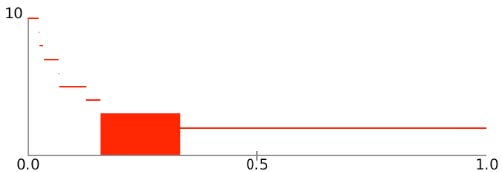
\includegraphics[width=\linewidth]{persistence-ui}
%     \caption{Persistence curve showing the number of partitions as a function of persistence.}
%     \label{fig:persistence-ui}
%     \end{center}
% \end{figure}

% \subsubsection{Topology-based analysis}
% \label{sec:persistence}

% Another approach is to compare two or more structures from different persistence levels and potentially use animations to help understand the changes.
% ?applications

% \subsubsection{Contour based}
% \todo{rephrase}
% Contour based approaches.
% Summaries:
% \begin{itemize}
% \item contour tree: n-dimensions data~\cite{carr03}. can be embedded in 2d. grow quickly which makes them  too large do display~\cite{carr10}.
% \item Reeb graph extend con-tour trees to more general manifolds, potentially creating loops 
% \item merge tree~\cite{pascucci07}
% \item topological spines~\cite{correa11} link together chains of critical points using canonical visual representations that preserve the topology and locality of extrema and the nesting structure of the surrounding contours.
% \end{itemize}

% These capture structures of a topology at a given level of simplification. They don't aim to help understand the simplification process though.

% \subsubsection{Morse Theory}
% \label{sec:morse}
% Morse~\cite{morse63}, Timo~\cite{bremer04}, etc.

% Gradient based structure.

% \begin{figure}[htb]
%     \begin{center}
%      \includegraphics[width=\linewidth]{morse}
%     \caption{Morse and Morse-Smale complexes}
%     \label{fig:morse}
%     \end{center}
% \end{figure}

% \subsubsection{Morse Smale Simplification}
% ~\cite{bremer05}
% Simplifying MSC by canceling pairs of critical points. Both to address noise in the data and to create a simpler representation. 

% Persistence diagrams provide and overall view of all the critical points but without connectivity between points.Do not address hierarchical MSC approximations.



    
% \subsection{GERBER'S WORK}
% \label{sec:inverse-curves}

% \todo[inline]{Gerber used them for both the 1D projection plots and for the 3D summary. We use them in the plots as well and for sampling but we won't be talking about sampling here. Need to decide how much to talk about them and how best to describe their benefits in the plots (Regulus's details view)}

% To summarise the behaviour of the function within each partition we compute an inverse regression curve, that is a curve that maps from the scalar function range back to the d-dimensions domain. In particular, we use locally weighted regression (LOWESS)~\cite{Cleveland88}.

% \todo[inline]{the following is too long}
% kernel regression
% \[ f(x) = E[y|x] = \int y p(y|x) dy = \frac{\int y p(x,y) dy}{\int p(x,y) dy} \]
% using a Gaussian kernel 
% \[ f(x) = \sum_{i=1}^N y_i \frac{k(x, x_i)}{\sum_{j=1}^N k(x, x_j)} \]
% which is essentially fitting a constant function locally. We then fit a linear regression model for each point x by solving,
% \[ \min_{\beta(x)}\sum_{i=1}^N k(x, x_i)[y_i - \beta(x)^T\phi(x_i)]^2 \]
% where $\phi(x) = [1, x]$.
% We can then compute the parameters $\beta(x)$ by solving the weighted least square problem
% \[ \beta(x) = (\Phi^TD(x)\Phi)^{-1}\Phi^TD(x_y \]

% \begin{itemize}
%     \item \textit{"Principal curves are smooth one-dimensional curves that pass through the middle of a p-dimensional dataset, providing a nonlinear summary of the data.They are non-parametric, and their shape is suggested by the data"}~\cite{Tibshirani92}
%     \item Gerber~\cite{Gerber10} employed inverse regression curves based on locally weighted regression (LOWESS)~\cite{Cleveland88}. He used the mean std to define a hyper tube around the inverse curve (hyper circle with radium = mean std).
% \end{itemize}

% Gerber used the inverse regression curves to provide a geometric summary of a partition. For a given persistence level, Gerber displayed the inverse curves after projecting them to a 3D using PCA. This presentation often lead to confusion by users as they tried to assign meaning to the shape of the curves in 3D.
